\documentclass[a4paper,12pt]{article}
%\documentclass[a4paper,10pt]{scrartcl}

\usepackage[utf8]{inputenc}
\usepackage[english]{babel}
\usepackage[pdftex]{graphicx}
\usepackage{amssymb}
\usepackage{marvosym}
\usepackage{amsmath}
\usepackage{array}
\usepackage{geometry}

\geometry{verbose,tmargin=1cm,headheight=80pt,lmargin=2cm,bmargin=4cm,rmargin=2.5cm}

\title{Exercise 2 - Solution}
\author{}
\date{}

\pdfinfo{%
  /Title    ()
  /Author   ()
  /Creator  ()
  /Producer ()
  /Subject  ()
  /Keywords ()
}

\begin{document}
\maketitle

\section*{Task 2.1}

given : $a = 58000km,\epsilon = 0.7, i = 51^{\circ}, \mu_E = 3.986\cdot 10^5 \frac{km^3}{s^2}, J_2 = 1082.7 \cdot 10^{-6}, t_{Earth} = 24h$

\noindent to be determined: $T, r_a, r_p, \Delta\Omega, \Delta\omega$
\begin{enumerate}
 \item \[ T = 2\pi\sqrt{\frac{a^3}{\mu_E}} = 139012.2944s = 2316.87 min\]
 \item \[ r_a = a(1+\epsilon) = 17400km\]
 \[r_p = a(1-\epsilon) = 98600km\]
 \item \[\Delta\Omega = - \frac{3\pi J_2R_E^2}{a^2(1-\epsilon^2)^2}cos(i)\cdot \frac{t_{Earth}}{T} = -1.86\cdot 10^{-4} \frac{rad}{day} \approx 0.0106 \frac{deg}{day}\]
 \[\Delta\omega = \frac{3\pi J_2R_E^2}{2a^2(1-\epsilon^2)^2}(4-5sin^2(i))\cdot \frac{t_{Earth}}{T} = 1.4451 \cdot 10^{-4}\frac{rad}{day} \approx 0.0083 \frac{deg}{day}\]
\end{enumerate}


\section*{Task 2.2}
given: $i = 97.76^{\circ}, \epsilon = 0.0063, \Omega = 352.26^{\circ}, T = 97.7min, \omega = 213.57^{\circ}, \nu = 146.03^{\circ}$

\noindent to be determined: $a, \text{average angular velocity}, lat_{SSP}, long_{SSP}$
\\SSP = subsatellite point
\begin{enumerate}
 \item \[ a = \sqrt[3]{\frac{T^2}{4\pi^2}\cdot \mu_E} = 7026.78 km\]
 \item \[ \text{average angular velocity} = \frac{2\pi}{T} = \frac{360^{\circ}}{T} = 3.685 \frac{deg}{min}\]
 \item \[ lat_{SSP} = arcsin\left(sin(i)\cdot sin(\nu+\omega)\right) = -0.4^{\circ} \]
 \[long_{SSP} = arccos\left(\frac{cos(\nu+\omega)}{cos(lat_{SSP})}\right) + \Omega + \lambda_{greenwich}= 681.01^{\circ} = -38.99^{\circ}\]
\end{enumerate}

\section*{Task 2.3}
given: $a = 26562km, \epsilon = 0.77, i = 63.4^{\circ}$ 

\noindent to be determined: $\Delta \Omega, \Delta \Phi$

\begin{enumerate}
 \item $J_2$ decreases the value of $\Delta \Omega$ \[\Delta\Omega = -\frac{3\pi J_2R_E^2}{a^2(1-\epsilon^2)^2}cos(i) = -0.0015895 \frac{rad}{rev} = -0.09107 \frac{deg}{rev}\]
 \item \[T = 2\pi\sqrt{\frac{a^3}{\mu_E}} = 718.044 min =  \frac{718.044}{23\cdot60+56+4/60}\text{ sidereal days} = 0.5 \text{ sidereal days}\]
 \\ After 100 sidereal days: $\frac{100 \text{ sidereal days}}{T} = 200$ revolutions
 \[\Rightarrow \Delta \Omega_{100} = 200\ rev \cdot (-0.09107) \frac{deg}{rev} = -18.214 deg\]
\end{enumerate}

\begin{figure}[!ht]
 \centering
 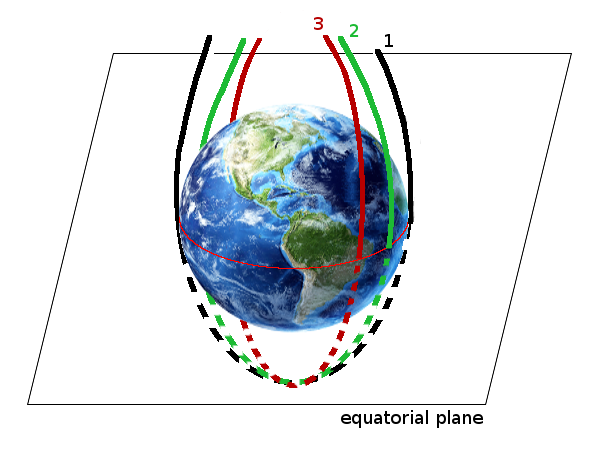
\includegraphics[scale=0.6]{../Loesungen/pic2}
\end{figure}


\end{document}
